\textbf{Motivation.} Before asking how fast agents' issues are closed or what they are about, a baseline is needed: how many issues each agent has, whether they get closed, how they are labelled, and how they are linked to the agent in the first place. Maintainers who consider adopting an agent face the same questions.

\textbf{Approach.} Metrics M1.1--M1.10 were computed for every agent (Table~\ref{tab:rq1}), and five associations were tested between the agent and a category (state, closure reason, labelled or not, language group and attribution signal) on the eleven tested agents. Adjusted residuals then show which agents drive each association. For the two agents with both bot-written and other issues, CodeRabbit and Devin, closure rates were compared within the agent with a two-proportion test, Newcombe intervals for the difference~\cite{newcombe1998interval} and Cohen's \(h\)~\cite{cohen1988power}.

\begin{table}[t]
\caption{Agent profile (RQ1). Closed, Labelled, Non-En.\ (not English) and Own bot are \% of the agent's issues; NP = closed as not planned, \% of closed issues}\label{tab:rq1}
\centering\footnotesize\setlength{\tabcolsep}{3pt}
\resizebox{\columnwidth}{!}{\begin{tabular}{@{}lrrrrrrr@{}}
\toprule
Agent & Issues & Repos & Closed & NP & Labelled & Non-En. & Own bot\\
\midrule
\inputtab{generated/tab_rq1_profile.tex}
\bottomrule
\multicolumn{8}{@{}l}{\scriptsize $^\dagger$Descriptive only (three issues each).}
\end{tabular}}
\end{table}

\textbf{Results.} \emph{Volume and spread.} Three agents dominate the data: CodeRabbit, Claude Code and Sweep account for \TopThreeShare\% of all issues, while the five smallest tested agents have fewer than 110 issues each. The issues are spread thinly over many repositories. Every tested agent has a median of one issue per repository, and no single repository holds more than \TopRepoMax\% of any tested agent's issues, so no project dominates an agent's profile; the Gini coefficient of each agent's issues over repositories ranges from \GiniMin{} (\GiniMinAgent) to \GiniMax{} (\GiniMaxAgent). Closure rates vary widely, from \ClosedMin\% for \ClosedMinAgent{} (95\% CI \ClosedMinCI) to \ClosedMax\% for \ClosedMaxAgent{} (95\% CI \ClosedMaxCI).

\emph{Associations.} All five associations are significant after Holm correction (\(p_{\text{perm}} \le 0.001\)), but their strength differs a great deal. The agent is weakly associated with state (V = \VState, \EffState), closure reason (V = \VReason, \EffReason) and language (V = \VLanguage, \EffLanguage), moderately with labelling (V = \VLabelled, \EffLabelled; on average an issue carries from \LabelsMeanMin{} labels for \LabelsMeanMinAgent{} to \LabelsMeanMax{} for \LabelsMeanMaxAgent), and strongly with the attribution signal (V = \VAttribution, \EffAttribution). The clearest difference between agents, then, is not what happens to their issues but how the issues are tied to them in the first place (Fig.~\ref{fig:rq1attr}). For CodeRabbit (\OwnBotShareCoderabbit\%) and Devin (\OwnBotShareDevin\%), the agent's own bot account wrote most issues. For Claude Code, Sweep and Jules, almost none were bot-written: a human opened the issue and the agent is triggered, mentioned or credited in the text. The manual check of a random sample of 99 issues shows how varied these links are: of the issues that are really linked to their agent, the agent wrote \ValRoleWPct\%, a person triggered the agent in \ValRoleTPct\%, and in \ValRoleMPct\% the agent is only mentioned or discussed. Language differs as well: \NonEnDevin\% of Devin's issues are not in English, against \NonEnSweep\% of Sweep's.

\begin{figure*}[t]
\centering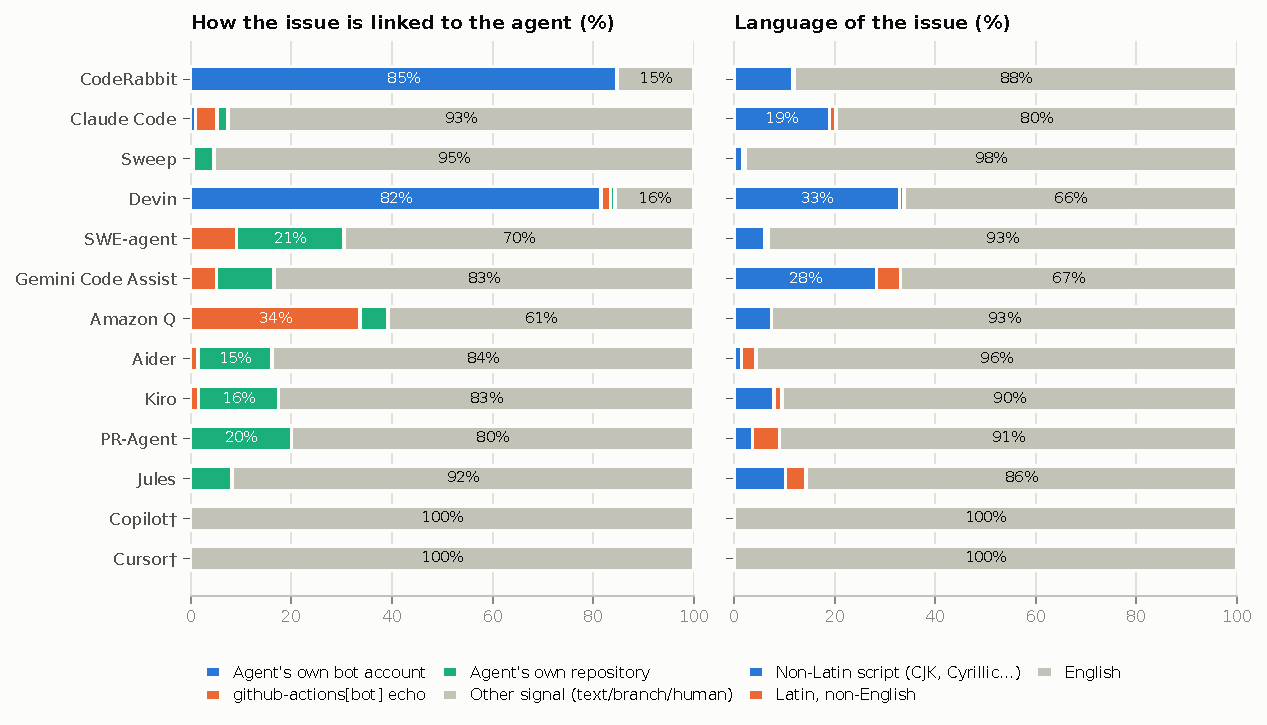
\includegraphics[width=0.86\textwidth]{rq1_F3_attribution_language.pdf}
\caption{How each agent's issues are linked to the agent (left) and their language (right).}\label{fig:rq1attr}
\end{figure*}

\emph{Agent-written issues stay open.} The role of the agent turns out to matter for whether an issue is closed. Within the same agent, issues written by the agent's own bot are closed less often than issues linked to the agent in other ways (Table~\ref{tab:fa}): \DiffCoderabbit{} percentage points for CodeRabbit (95\% CI \DiffCICoderabbit; \(h = \HCoderabbit\), \HEffCoderabbit) and \DiffDevin{} points for Devin (95\% CI \DiffCIDevin; \(h = \HDevin\), \HEffDevin), both significant after Holm correction. Issue age is an obvious alternative explanation, but it does not hold: the bot-written issues are \emph{older} (median \AgeOwnCoderabbit{} against \AgeOtherCoderabbit{} days for CodeRabbit), so they have had more time to be closed, and among issues at least 180 days old the gaps hardly change (\DiffOldCoderabbit{} and \DiffOldDevin{} points). Across all agents, \OwnClosedAll\% of bot-written and \OtherClosedAll\% of other issues are closed. The bot-written issues of the two agents are of different kinds. CodeRabbit's are follow-ups from its reviews (\OwnPRRefAllCoderabbit\% refer to a pull request or review), whereas Devin's mostly describe new tasks (\OwnPRRefAllDevin\%). For CodeRabbit, a plausible reading is that maintainers treat review follow-ups as lower-priority suggestions, in line with developers' reports that unsolicited bot activity feels like noise~\cite{wessel2021disturb}. The data show the association, not its cause.

\begin{table}[t]
\caption{Closure rate (\%, Wilson 95\% CI) of issues written by the agent's own bot and of the agent's other issues}\label{tab:fa}
\centering\footnotesize\setlength{\tabcolsep}{3pt}
\resizebox{\columnwidth}{!}{\begin{tabular}{@{}lccccc@{}}
\toprule
Agent & Own bot & Other & Diff.\ (pp) & z & p\\
\midrule
CodeRabbit & \OwnClosedCoderabbit{} \OwnCICoderabbit & \OtherClosedCoderabbit{} \OtherCICoderabbit & \DiffCoderabbit & \ZCoderabbit & $\PCoderabbit$\\
Devin & \OwnClosedDevin{} \OwnCIDevin & \OtherClosedDevin{} \OtherCIDevin & \DiffDevin & \ZDevin & $\PDevin$\\
\bottomrule
\end{tabular}}
\end{table}

\emph{The labelling illusion.} Labels are GitHub's built-in way to classify and triage issues, and how projects use them is associated with how issues are resolved~\cite{cabot2015labels}. By the usual measure, Sweep is the most-labelled tested agent: \SweepAnyLabel\% of its issues carry a label (95\% CI \SweepAnyLabelCI). Most of these labels, however, are \texttt{sweep} itself (\SweepLabelShare\% of all labels on Sweep's issues), the label a user adds to invoke the agent. Counting only labels that classify the work, Sweep falls to \SweepTriageLabel\% and ranks last of all thirteen agents, a drop of \SweepDrop{} points. Amazon Q (\(-\)\AmazonQDrop{} points) and Jules (\(-\)\JulesDrop) drop too, while no other agent changes by more than \OtherMaxDrop{} points. For trigger-based agents, a label therefore records how the agent was called, not how maintainers organise the work. This adds a new source of noise to labels that are already known to be unreliable as an issue classification~\cite{herzig2013bug}.

\rqsummary{RQ1}{Agents differ most in how their issues are linked to them. For CodeRabbit and Devin, most issues were written by the agent's own bot, and these issues are closed 18--24 percentage points less often than the same agents' other issues, a gap that issue age does not explain. For trigger-based agents such as Sweep, most labels invoke the agent rather than classify the work. Comparisons of ``agent issues'' should therefore separate the role of the agent and remove agent-workflow labels before using labels as data.}
